\clearpage
\section{Analyse}
\subsection{Genauigkeit und Verwendbarkeit der Daten}
\label{subsec:analyseprecision}
Die GPS Daten, die mit dem verwendeten Gerät (Google Nexus 5) aufgezeichnet wurden, sind - wie für GPS üblich \cite{gpsprecision} - bis auf wenige Meter genau. Die Genauigkeit hängt dabei vor Allem von der Umgebung ab. In Tunneln oder in engen Häuserschluchten ist der Empfang schlechter als auf einem offenen Feld oder im Wald. 

\begin{figure}[h]
  \centering
  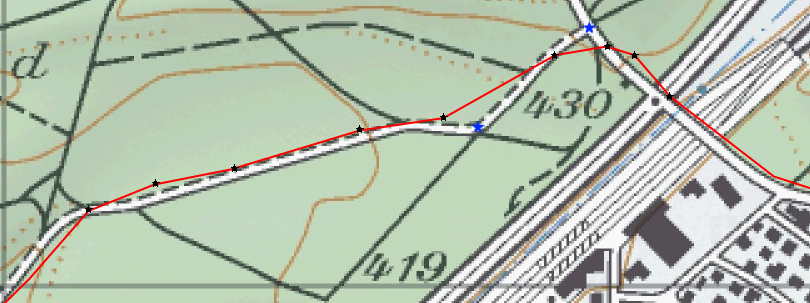
\includegraphics[width=\textwidth]{images/map_issues_10s.png}
  \caption[Genauigkeitsprobleme - zu wenige Datenpunkte]{Genauigkeitsprobleme - zu wenige Datenpunkte}
  \label{fig:precisionissues10s}
\end{figure}

Probleme durch diese Ungenauigkeit sind vor allem aufgetreten, wenn zu wenig Datenpunkte erfasst wurden. In der Abbildung \ref{fig:precisionissues10s} ist dies gut ersichtlich. Die schwarzen Sternchen stehen für GPS Datenpunkte. Das erste schwarze Sternchen von Rechts liegt ziemlich gut auf der Strasse. Das Zweite ist aufgrund der GPS Ungenauigkeiten und äusseren Einflüssen um einige Meter daneben. Das Dritte ist wieder korrekt auf der Strasse. Zwischen dem Dritten und Vierten bin ich von der Strasse auf einen Waldweg abgebogen. Der vierte Datenpunkt liegt schön auf diesem Waldweg, auf der Karte ist der Punkt an dem ich wirklich abgebogen bin (blauer Stern) nicht erfasst. Das Selbe geschieht zwischen dem vierten und fünften Datenpunkt. Diese Probleme liessen sich durch das Aufzeichnen von mehr Datenpunkten minimieren.

\begin{figure}[h]
  \centering
  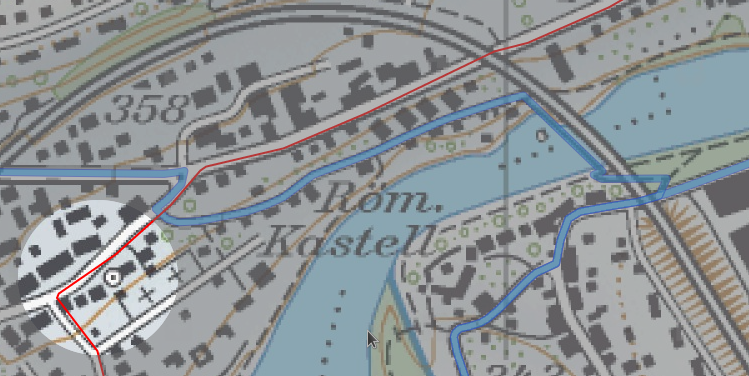
\includegraphics[width=0.9\textwidth]{images/map_issues_1s.png}
  \caption[GPS Ungenauigkeit]{GPS Ungenauigkeit}
  \label{fig:precisionissues1s}
\end{figure}

Bei einer genügenden Menge Datenpunkte wie in Abbildung \ref{fig:precisionissues1s} existieren immer noch Ungenauigkeiten. Die Route im markierten Bereich verläuft ein bis zwei Meter neben der Strasse. Jedoch wird hier im Gegensatz zur Abbildung \ref{fig:precisionissues10s} der Richtungswechsel problemlos korrekt eingezeichnet.

Man kann die Daten, sofern genügend Datenpunkte vorhanden sind, in der Form in welcher sie derzeit generiert werden durchaus verwenden um den Verlauf einer Fahrradtour festzuhalten. Die im Rahmen dieses Projektes aufgezeichneten Routen sind nicht befreit von Ungenauigkeiten, jedoch ist überall ersichtlich auf welcher Strasse ich gefahren bin. Um die vorhandenen Ungenauigkeiten zu minimieren, könnte man zum Beispiel einen  Map-Matching Filter anwenden wie er von Jason Daniel Martin et al. im Paper Dynamic GPS-position correction for mobile pedestrian navigation and orientation \cite{gpscorrection} vorgestellt wird. Um die Anzahl Datenpunkte zu verkleinern und um Ausreisser zu eliminieren könnten numerische Verfahren wie zum Beispiel der Ramer-Douglas-Peucker Algorithmus \cite{ramer}\cite{douglaspeucker} verwendet werden.

Die Aufgezeichneten Höhen (Altitude), beziehungsweise deren Differenzen weichen in allen Messungen sehr stark von der Realität ab. Auf der Karte von Schweizmobil\cite{velolandmap} können bei Bedarf korrekte Angaben zur Höhendifferenz ausgelesen werden.

\subsection{Akkuverbrauch}
\label{subsec:analysebatteryusage}
Mit dem Java Android SDK ist es nicht möglich den Akkuverbrauch einer einzelnen Applikation zu messen. Was möglich ist, ist das Messen des aktuellen Akkustandes. In dem erstellen GPS Tracker wurde dies jeweils beim Start und nach Abschluss jedes Tracks getan. Die Auflösung dieser Messwerte sind auf 0.01 oder 1\% des Akkus genau.

Die Eingabeparameter des \lstinline$LocationManagers$ welche einen Einfluss auf den Akkuverbrauch des Trackers haben könnten, sind die im Kapitel \ref{subsec:programmlogikbackend} beschriebenen:
\begin{itemize}
	\item timeInterval
	\item minDistance
\end{itemize}

Wirklich relevant hierbei ist lediglich das \lstinline$timeInterval$. In diesen Abständen wird die GPS Location abgerufen. Um den Einfluss dieser Einstellung auf den Akkuverbrauch zu messen, wurden über rund drei Stunden Tracks mit verschiedenen Zeitintervallen aufgenommen:

\begin{figure}[h]
  \centering
  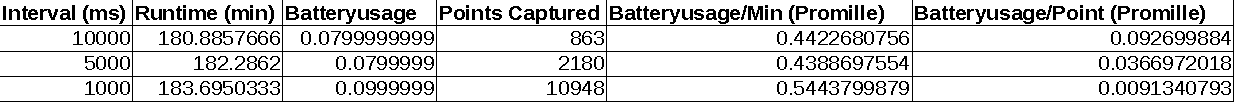
\includegraphics[width=\textwidth]{images/batteryusage.pdf}
  \caption[Statistik Akkuverbrauch]{Statistik Akkuverbrauch}
  \label{fig:batteryusage}
\end{figure}

In der Abbildung \ref{fig:batteryusage} sind die Resultate dieses Tests ersichtlich. Es hat sich kein markanter Unterschied des Akkuverbrauchs aufgrund dieser Konfigurationsparameter feststellen lässt. Dies deckt sich mit der Stackexchange Antwort vom Stackexchange User Jan:

\flqq ...Your 10 second time value might be used by the OS to control power usage, but there is no guarantee. And, with that low of a value, it seems highly unlikely that it would be used. Every hour, maybe, but not every 10 seconds.

The bigger thing is that you will be needing to keep the CPU powered on all the time. And, since you're using the PendingIntent flavor of requestLocationUpdates(), I am guessing that you plan on collecting data for a long time....\frqq \cite{batteryusage}

Er beschreibt, dass das Hauptproblem das ständige Arbeiten des Prozessors sei, welches zum Tracken der Location notwendig ist. Gemäss ihm sei es vor allem wichtig, dass man die \lstinline$LocationUpdates$ wieder ausschaltet wenn man sie nicht mehr braucht. Dies ist der Fall in dem hier hergestellten GPS Tracker.